\subsection{Buck-boost converter}

\subsubsection{init - configuracoes da simulacao}

The values used to simulate the Buck-boost converter example are:

- $\Omega$: $\Big[1, 2\Big]$

- $s_{max}$ is set to 2.

- The dynamics of the system are defined by

\begin{equation}
    \begin{matrix}
        A_1 = \left[ \begin{matrix} 0 & 0 \\ 0 & -1/(RC) \\ \end{matrix} \right] &
        A_2 = \left[ \begin{matrix} 0 & 1/L \\ -1/C & -1/(RC) \\ \end{matrix} \right] \\
        \\
        b_1 = \left[ \begin{matrix} E/L \\ 0 \end{matrix} \right] &
        b_2 = \left[ \begin{matrix} 0 \\ 0 \end{matrix} \right]
    \end{matrix}
\end{equation}

\noindent
where R = 1, L = 1, C = 1, E = 1.

- $t_{step}$ is set to 1e-5.

- $x_{ref}$ is set to [2, -1].

- $Q$ which is a diagonal matrix with both diagonal elements equal to 1.

- $T_{p_{max}}$ set to 1.

- $T_{s}$ defined as [0, 0.2513520, 0.5914520].

- $x_{0}$ set to [1.870801, -1.119853].


\subsubsection{calculo da trajetoria (optimizacao)}

\begin{equation}
    T_{s} = 
    \left[
    \begin{matrix}
        0 & 0.2500021 & 0.5004299
    \end{matrix}
    \right]
\end{equation}


\subsubsection{construindo MPC (matrizes PHI e GAMMA)}


\begin{equation}
    \Phi =
    \left[
    \begin{matrix}
        1 & 0 \\
        0 &0.7788 
    \end{matrix}
    \right]
\end{equation}

\begin{equation}
    \Gamma =
    \left[
    \begin{matrix}
        1 \\
        1.1108 
    \end{matrix}
    \right]
\end{equation}

\subsubsection{rodando simulacao}


time constraints:

\begin{equation}
    c = 
    \left[
        \begin{matrix}
            \Delta t_{r_1} -\Delta t_{r_{1, min}} \\
            \Delta t_{r_2} -\Delta t_{r_{2, min}} \\
            \vdots \\
            \Delta t_{r_{N-1}} -\Delta t_{r_{{N-1}, min}} \\
            \Delta t_{r_N} -\Delta t_{r_{N, min}} \\
        \end{matrix}
    \right] = 
    \left[
        \begin{matrix}
            - 0.25 + 0.25 \\
            - 0.2504 + 0.25 \\
        \end{matrix}
    \right] =
    \left[
        \begin{matrix}
            0 \\
            - 0.04 \\
        \end{matrix}
    \right]
\end{equation}

\subsubsection{resultados}

\begin{figure}[h]
    \centering
    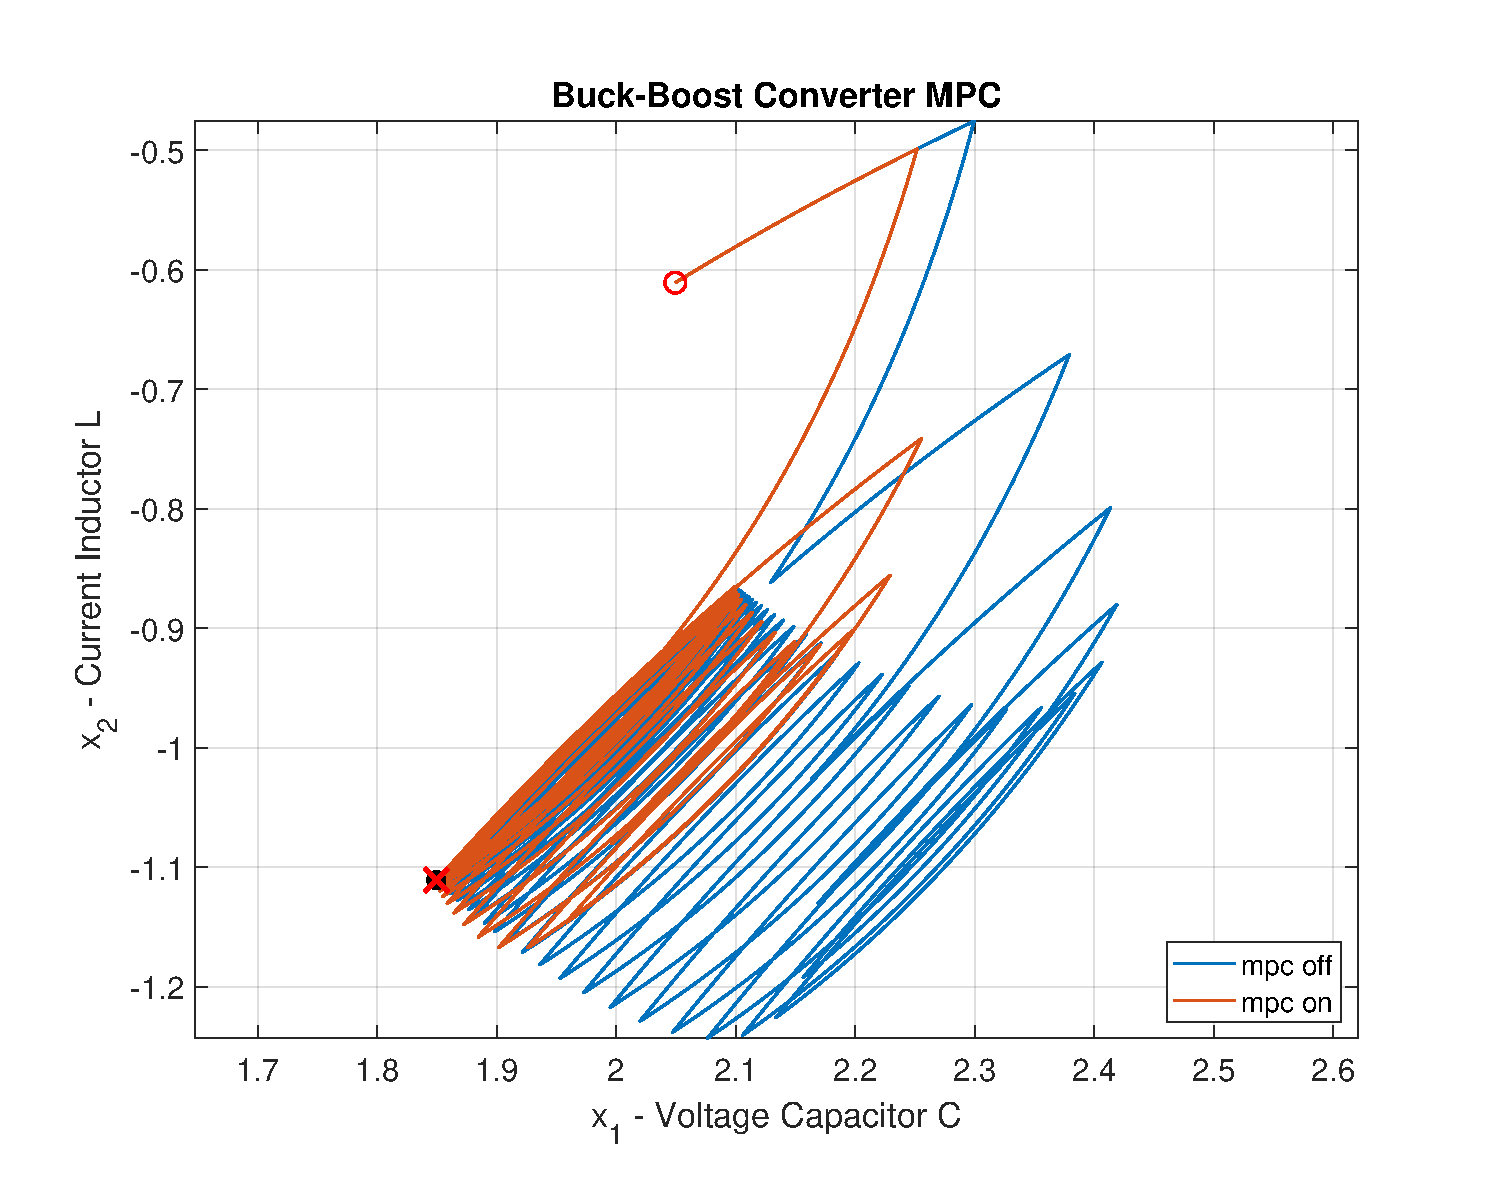
\includegraphics[width=14cm]{Cap4/fig/graf_patino_ex1_1.pdf}
    \caption{fig 1}
    \label{cap4-graf-patino-ex1-1}
\end{figure}

\begin{figure}[h]
    \centering
    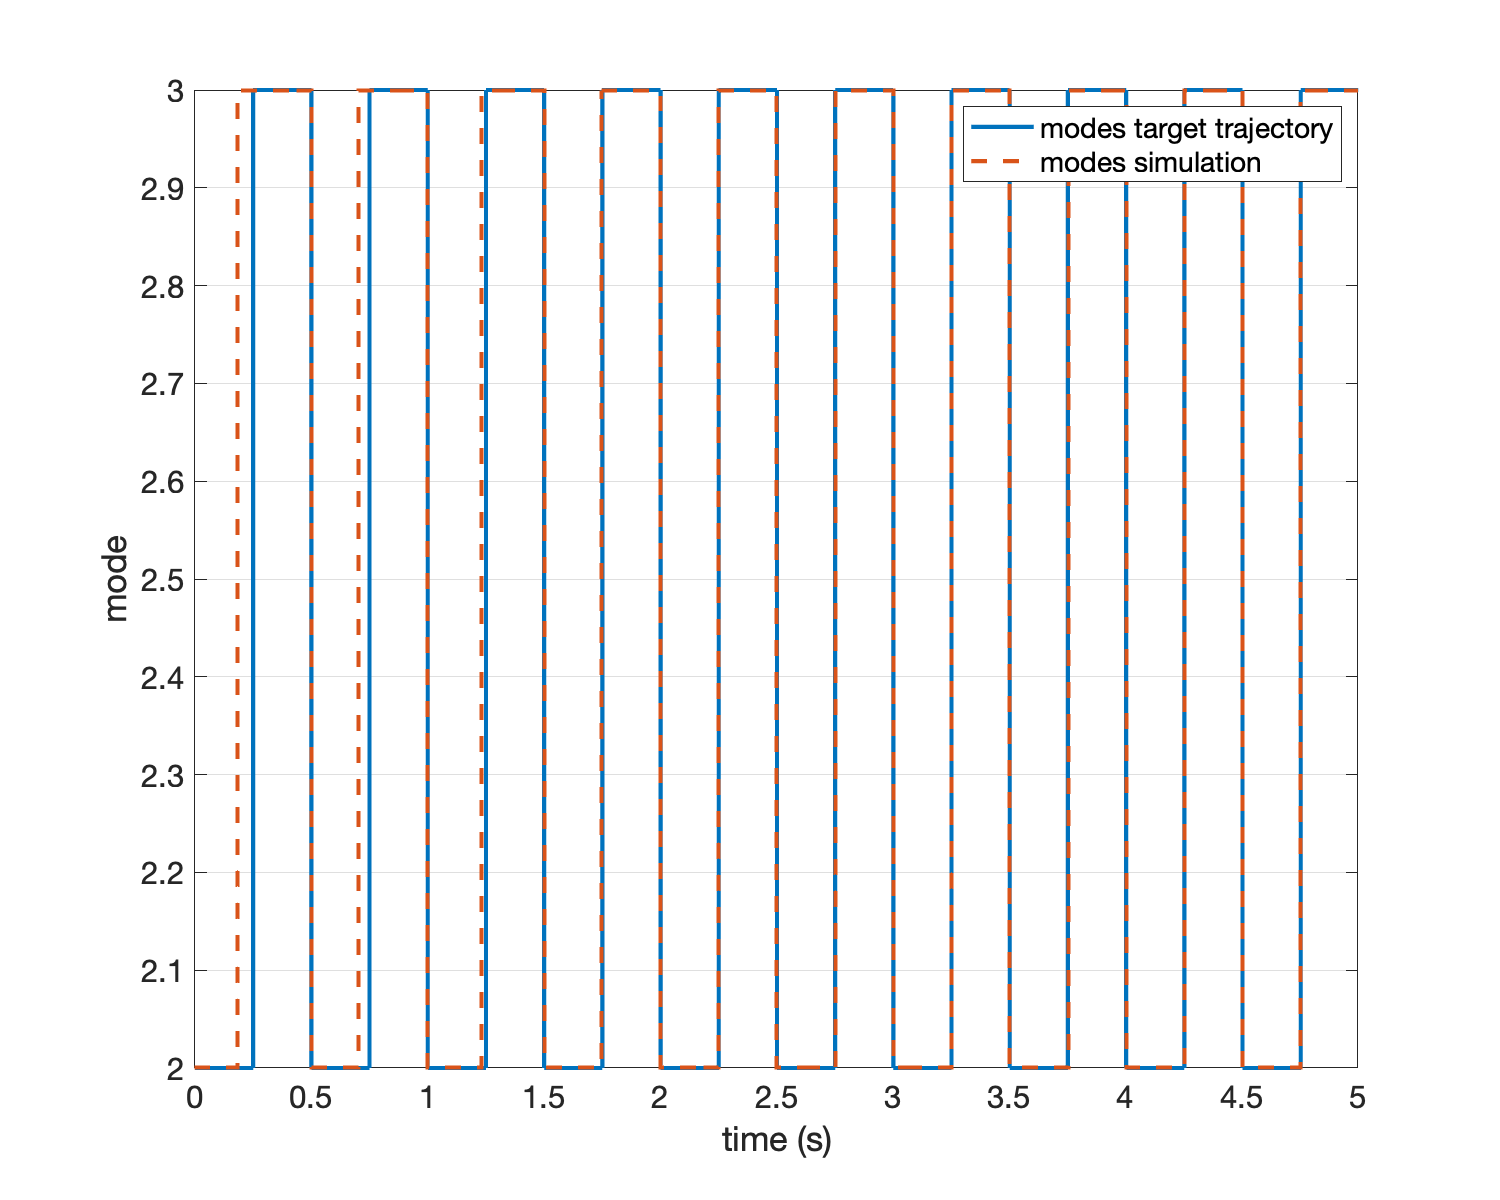
\includegraphics[width=14cm]{Cap4/fig/graf_patino_ex1_2.pdf}
    \caption{fig 2}
    \label{cap4-graf-patino-ex1-2}
\end{figure}
